\documentclass{standalone}
\usepackage{tikz}
\usetikzlibrary{patterns, positioning}


\begin{document}
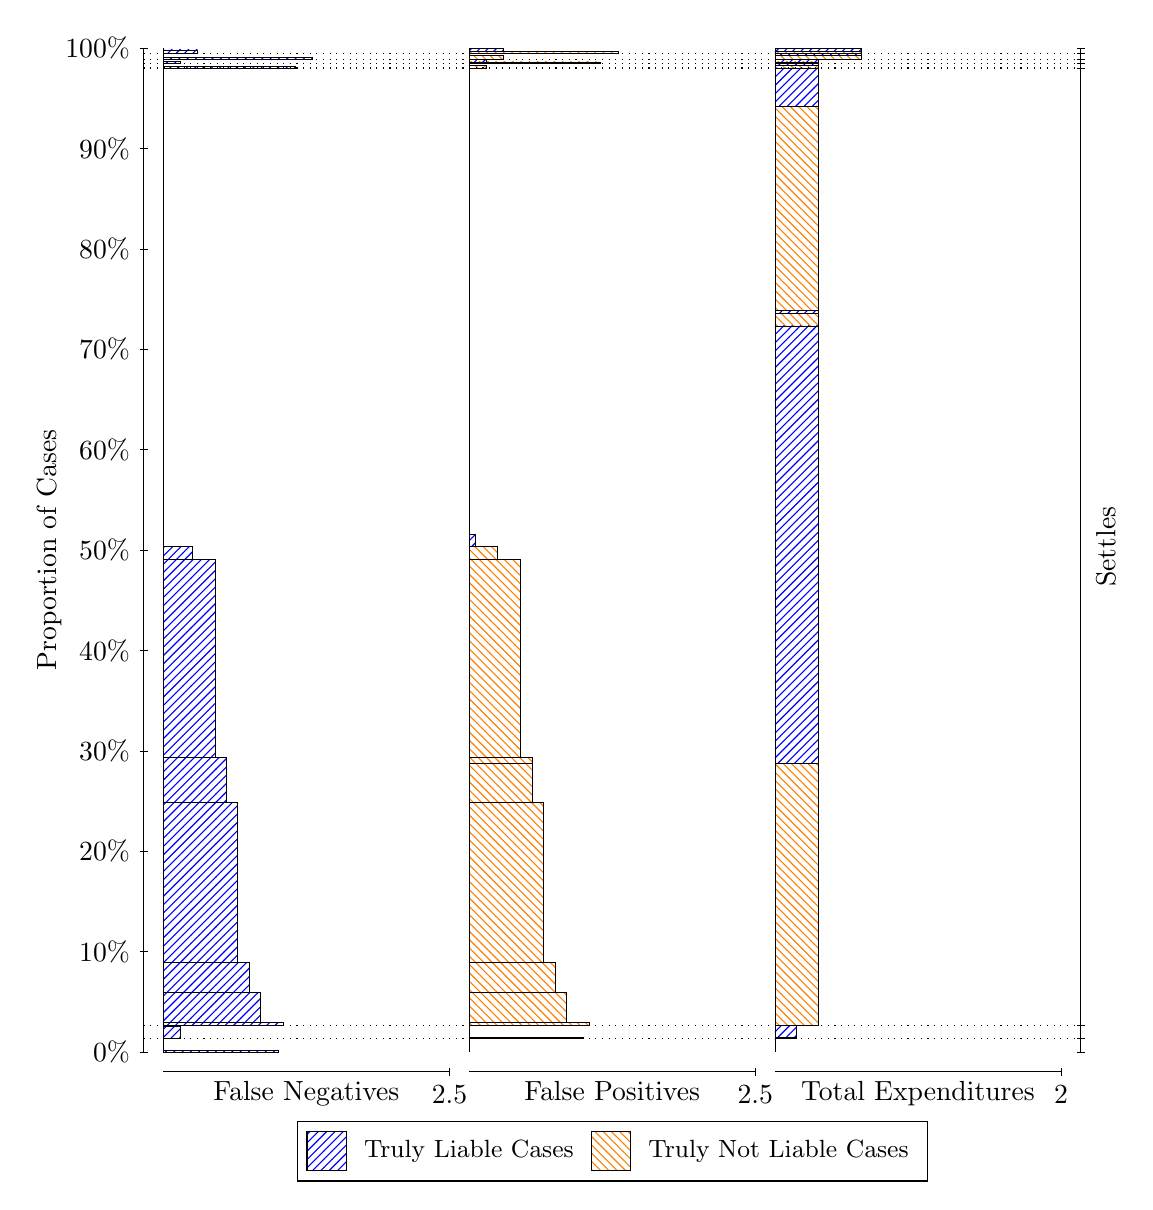
\begin{tikzpicture}
\draw[black, very thin] (1.5,1.75) -- (1.5,14.5);
\node[rotate=90, text=black, anchor=center] at (0.3, 8.125) {Proportion of Cases};
\draw[black, very thin] (1.45,1.75) -- (1.55,1.75);
\node[text=black, anchor=east] at (1.45, 1.75) {0\%};
\draw[black, very thin] (1.45,3.025) -- (1.55,3.025);
\node[text=black, anchor=east] at (1.45, 3.025) {10\%};
\draw[black, very thin] (1.45,4.3) -- (1.55,4.3);
\node[text=black, anchor=east] at (1.45, 4.3) {20\%};
\draw[black, very thin] (1.45,5.575) -- (1.55,5.575);
\node[text=black, anchor=east] at (1.45, 5.575) {30\%};
\draw[black, very thin] (1.45,6.85) -- (1.55,6.85);
\node[text=black, anchor=east] at (1.45, 6.85) {40\%};
\draw[black, very thin] (1.45,8.125) -- (1.55,8.125);
\node[text=black, anchor=east] at (1.45, 8.125) {50\%};
\draw[black, very thin] (1.45,9.4) -- (1.55,9.4);
\node[text=black, anchor=east] at (1.45, 9.4) {60\%};
\draw[black, very thin] (1.45,10.675) -- (1.55,10.675);
\node[text=black, anchor=east] at (1.45, 10.675) {70\%};
\draw[black, very thin] (1.45,11.95) -- (1.55,11.95);
\node[text=black, anchor=east] at (1.45, 11.95) {80\%};
\draw[black, very thin] (1.45,13.225) -- (1.55,13.225);
\node[text=black, anchor=east] at (1.45, 13.225) {90\%};
\draw[black, very thin] (1.45,14.5) -- (1.55,14.5);
\node[text=black, anchor=east] at (1.45, 14.5) {100\%};

\draw[black, very thin] (13.4,1.75) -- (13.4,14.5);
\draw[black, very thin] (13.35,1.75) -- (13.45,1.75);
\node[anchor=west] at (13.35, 1.75) {};
\draw[black, very thin] (13.35,1.9195) -- (13.45,1.9195);
\node[anchor=west] at (13.35, 1.9195) {};
\draw[black, very thin] (13.35,2.0889) -- (13.45,2.0889);
\node[anchor=west] at (13.35, 2.0889) {};
\draw[black, very thin] (13.35,14.247) -- (13.45,14.247);
\node[anchor=west] at (13.35, 14.247) {};
\draw[black, very thin] (13.35,14.302) -- (13.45,14.302);
\node[anchor=west] at (13.35, 14.302) {};
\draw[black, very thin] (13.35,14.357) -- (13.45,14.357);
\node[anchor=west] at (13.35, 14.357) {};
\draw[black, very thin] (13.35,14.428) -- (13.45,14.428);
\node[anchor=west] at (13.35, 14.428) {};
\draw[black, very thin] (13.35,14.5) -- (13.45,14.5);
\node[anchor=west] at (13.35, 14.5) {};

\draw[black, very thin, pattern color=blue, pattern=north east lines] (1.75,1.75) rectangle (3.2033,1.7678);
\draw[black, very thin, pattern color=orange, pattern=north west lines] (1.75,1.7678) rectangle (1.75,1.9195);
\draw[black, very thin, pattern color=blue, pattern=north east lines] (1.75,1.9195) rectangle (1.968,2.0711);
\draw[black, very thin, pattern color=orange, pattern=north west lines] (1.75,2.0711) rectangle (1.75,2.0889);
\draw[black, very thin, pattern color=blue, pattern=north east lines] (1.75,2.0889) rectangle (3.276,2.1236);
\draw[black, very thin, pattern color=blue, pattern=north east lines] (1.75,2.1236) rectangle (2.9853,2.506);
\draw[black, very thin, pattern color=blue, pattern=north east lines] (1.75,2.506) rectangle (2.84,2.888);
\draw[black, very thin, pattern color=blue, pattern=north east lines] (1.75,2.888) rectangle (2.6947,4.919);
\draw[black, very thin, pattern color=blue, pattern=north east lines] (1.75,4.919) rectangle (2.5493,5.4952);
\draw[black, very thin, pattern color=blue, pattern=north east lines] (1.75,5.4952) rectangle (2.404,8.0099);
\draw[black, very thin, pattern color=blue, pattern=north east lines] (1.75,8.0099) rectangle (2.1133,8.1679);
\draw[black, very thin, pattern color=orange, pattern=north west lines] (1.75,8.1679) rectangle (1.75,14.247);
\draw[black, very thin, pattern color=blue, pattern=north east lines] (1.75,14.247) rectangle (3.4213,14.27);
\draw[black, very thin, pattern color=orange, pattern=north west lines] (1.75,14.27) rectangle (1.75,14.302);
\draw[black, very thin, pattern color=blue, pattern=north east lines] (1.75,14.302) rectangle (1.968,14.334);
\draw[black, very thin, pattern color=orange, pattern=north west lines] (1.75,14.334) rectangle (1.75,14.357);
\draw[black, very thin, pattern color=blue, pattern=north east lines] (1.75,14.357) rectangle (3.6393,14.381);
\draw[black, very thin, pattern color=orange, pattern=north west lines] (1.75,14.381) rectangle (1.75,14.428);
\draw[black, very thin, pattern color=blue, pattern=north east lines] (1.75,14.428) rectangle (2.186,14.475);
\draw[black, very thin, pattern color=orange, pattern=north west lines] (1.75,14.475) rectangle (1.75,14.5);
\draw[black, very thin, pattern color=orange, pattern=north west lines] (5.6333,1.75) rectangle (5.6333,1.9016);
\draw[black, very thin, pattern color=blue, pattern=north east lines] (5.6333,1.9016) rectangle (5.6333,1.9195);
\draw[black, very thin, pattern color=orange, pattern=north west lines] (5.6333,1.9195) rectangle (7.0867,1.9373);
\draw[black, very thin, pattern color=blue, pattern=north east lines] (5.6333,1.9373) rectangle (5.6333,2.0889);
\draw[black, very thin, pattern color=orange, pattern=north west lines] (5.6333,2.0889) rectangle (7.1593,2.1236);
\draw[black, very thin, pattern color=orange, pattern=north west lines] (5.6333,2.1236) rectangle (6.8687,2.506);
\draw[black, very thin, pattern color=orange, pattern=north west lines] (5.6333,2.506) rectangle (6.7233,2.888);
\draw[black, very thin, pattern color=orange, pattern=north west lines] (5.6333,2.888) rectangle (6.578,4.9191);
\draw[black, very thin, pattern color=orange, pattern=north west lines] (5.6333,4.9191) rectangle (6.4327,5.412);
\draw[black, very thin, pattern color=orange, pattern=north west lines] (5.6333,5.412) rectangle (6.4327,5.4953);
\draw[black, very thin, pattern color=orange, pattern=north west lines] (5.6333,5.4953) rectangle (6.2873,8.0101);
\draw[black, very thin, pattern color=orange, pattern=north west lines] (5.6333,8.0101) rectangle (5.9967,8.1681);
\draw[black, very thin, pattern color=blue, pattern=north east lines] (5.6333,8.1681) rectangle (5.706,8.3261);
\draw[black, very thin, pattern color=blue, pattern=north east lines] (5.6333,8.3261) rectangle (5.6333,14.247);
\draw[black, very thin, pattern color=orange, pattern=north west lines] (5.6333,14.247) rectangle (5.8513,14.279);
\draw[black, very thin, pattern color=blue, pattern=north east lines] (5.6333,14.279) rectangle (5.6333,14.302);
\draw[black, very thin, pattern color=orange, pattern=north west lines] (5.6333,14.302) rectangle (7.3047,14.324);
\draw[black, very thin, pattern color=blue, pattern=north east lines] (5.6333,14.324) rectangle (5.8513,14.357);
\draw[black, very thin, pattern color=orange, pattern=north west lines] (5.6333,14.357) rectangle (6.0693,14.403);
\draw[black, very thin, pattern color=blue, pattern=north east lines] (5.6333,14.403) rectangle (5.6333,14.428);
\draw[black, very thin, pattern color=orange, pattern=north west lines] (5.6333,14.428) rectangle (7.5227,14.453);
\draw[black, very thin, pattern color=blue, pattern=north east lines] (5.6333,14.453) rectangle (6.0693,14.5);
\draw[black, very thin, pattern color=orange, pattern=north west lines] (9.5167,1.75) rectangle (9.5167,1.9016);
\draw[black, very thin, pattern color=blue, pattern=north east lines] (9.5167,1.9016) rectangle (9.5167,1.9195);
\draw[black, very thin, pattern color=orange, pattern=north west lines] (9.5167,1.9195) rectangle (9.7892,1.9373);
\draw[black, very thin, pattern color=blue, pattern=north east lines] (9.5167,1.9373) rectangle (9.7892,2.0889);
\draw[black, very thin, pattern color=orange, pattern=north west lines] (9.5167,2.0889) rectangle (10.062,5.412);
\draw[black, very thin, pattern color=blue, pattern=north east lines] (9.5167,5.412) rectangle (10.062,10.972);
\draw[black, very thin, pattern color=orange, pattern=north west lines] (9.5167,10.972) rectangle (10.062,11.13);
\draw[black, very thin, pattern color=blue, pattern=north east lines] (9.5167,11.13) rectangle (10.062,11.164);
\draw[black, very thin, pattern color=orange, pattern=north west lines] (9.5167,11.164) rectangle (10.062,13.762);
\draw[black, very thin, pattern color=blue, pattern=north east lines] (9.5167,13.762) rectangle (10.062,14.247);
\draw[black, very thin, pattern color=orange, pattern=north west lines] (9.5167,14.247) rectangle (10.062,14.279);
\draw[black, very thin, pattern color=blue, pattern=north east lines] (9.5167,14.279) rectangle (10.062,14.302);
\draw[black, very thin, pattern color=orange, pattern=north west lines] (9.5167,14.302) rectangle (10.062,14.324);
\draw[black, very thin, pattern color=blue, pattern=north east lines] (9.5167,14.324) rectangle (10.062,14.357);
\draw[black, very thin, pattern color=orange, pattern=north west lines] (9.5167,14.357) rectangle (10.607,14.403);
\draw[black, very thin, pattern color=blue, pattern=north east lines] (9.5167,14.403) rectangle (10.607,14.428);
\draw[black, very thin, pattern color=orange, pattern=north west lines] (9.5167,14.428) rectangle (10.607,14.453);
\draw[black, very thin, pattern color=blue, pattern=north east lines] (9.5167,14.453) rectangle (10.607,14.5);
\draw[black, dotted] (1.5,1.9195) -- (13.4,1.9195);
\draw[black, dotted] (1.5,2.0889) -- (13.4,2.0889);
\draw[black, dotted] (1.5,14.247) -- (13.4,14.247);
\draw[black, dotted] (1.5,14.302) -- (13.4,14.302);
\draw[black, dotted] (1.5,14.357) -- (13.4,14.357);
\draw[black, dotted] (1.5,14.428) -- (13.4,14.428);
\draw[black, very thin] (1.75,1.5) -- (5.3833,1.5);
\node[text=black, anchor=north] at (3.5667, 1.5) {False Negatives};
\draw[black, very thin] (5.3833,1.45) -- (5.3833,1.55);
\node[text=black, anchor=north] at (5.3833, 1.45) {2.5};

\draw[black, very thin] (5.6333,1.5) -- (9.2667,1.5);
\node[text=black, anchor=north] at (7.45, 1.5) {False Positives};
\draw[black, very thin] (9.2667,1.45) -- (9.2667,1.55);
\node[text=black, anchor=north] at (9.2667, 1.45) {2.5};

\draw[black, very thin] (9.5167,1.5) -- (13.15,1.5);
\node[text=black, anchor=north] at (11.333, 1.5) {Total Expenditures};
\draw[black, very thin] (13.15,1.45) -- (13.15,1.55);
\node[text=black, anchor=north] at (13.15, 1.45) {2};



\node[text=black, centered, rotate=90] at (13.72, 8.168) {Settles};





\draw (7.449999999999999,1.5) node[draw=none] (baseCoordinate) {};
\begin{scope}[align=center]
        \matrix[scale=0.5, draw=black, below=0.5cm of baseCoordinate, nodes={draw}, column sep=0.1cm]{
            \node[rectangle, draw, minimum width=0.5cm, minimum height=0.5cm, pattern color=blue, pattern=north east lines] {}; &
            \node[draw=none, font=\small, text=black] (B) {Truly Liable Cases}; &
            \node[rectangle, draw, minimum width=0.5cm, minimum height=0.5cm, pattern color=orange, pattern=north west lines] {}; &
            \node[draw=none, font=\small, text=black] (B) {Truly Not Liable Cases}; \\
            };
\end{scope}

\end{tikzpicture}
\end{document}